\begin{rightcolumn}

\subsection{VALOR POTENCIAL CON EXPLOTACI\'ON DE OPORTUNIDADES EXTERNAS.}

Se utilizó una metodología de valuación de negocios basada en el punto número 4 del pentágono de explotación de oportunidades, conocido como \textit{valor con oportunidades externas}. (\autoref{fig:hexagono})\\

``\textcolor{secundario}{Valor potencial con explotaci\'on de oportunidades externas}.- Es el valor que adquiere la unidad econ\'omica valuada una vez que se realiz\'o la identificaci\'on y explotaci\'on de los factores externos. Para lo cual se corrigen deficiencias, se mejoran y optimizan procesos y se explotan nuevas oportunidades estrat\'egicas, obteni\'endose as\'i un mayor valor de la unidad econ\'omica''\\



\end{rightcolumn}
\begin{leftcolumn}

\begin{figure}[H]
\centering
\caption{Pent\'agono de Explotaci\'on de oportunidades\label{fig:hexagono}}
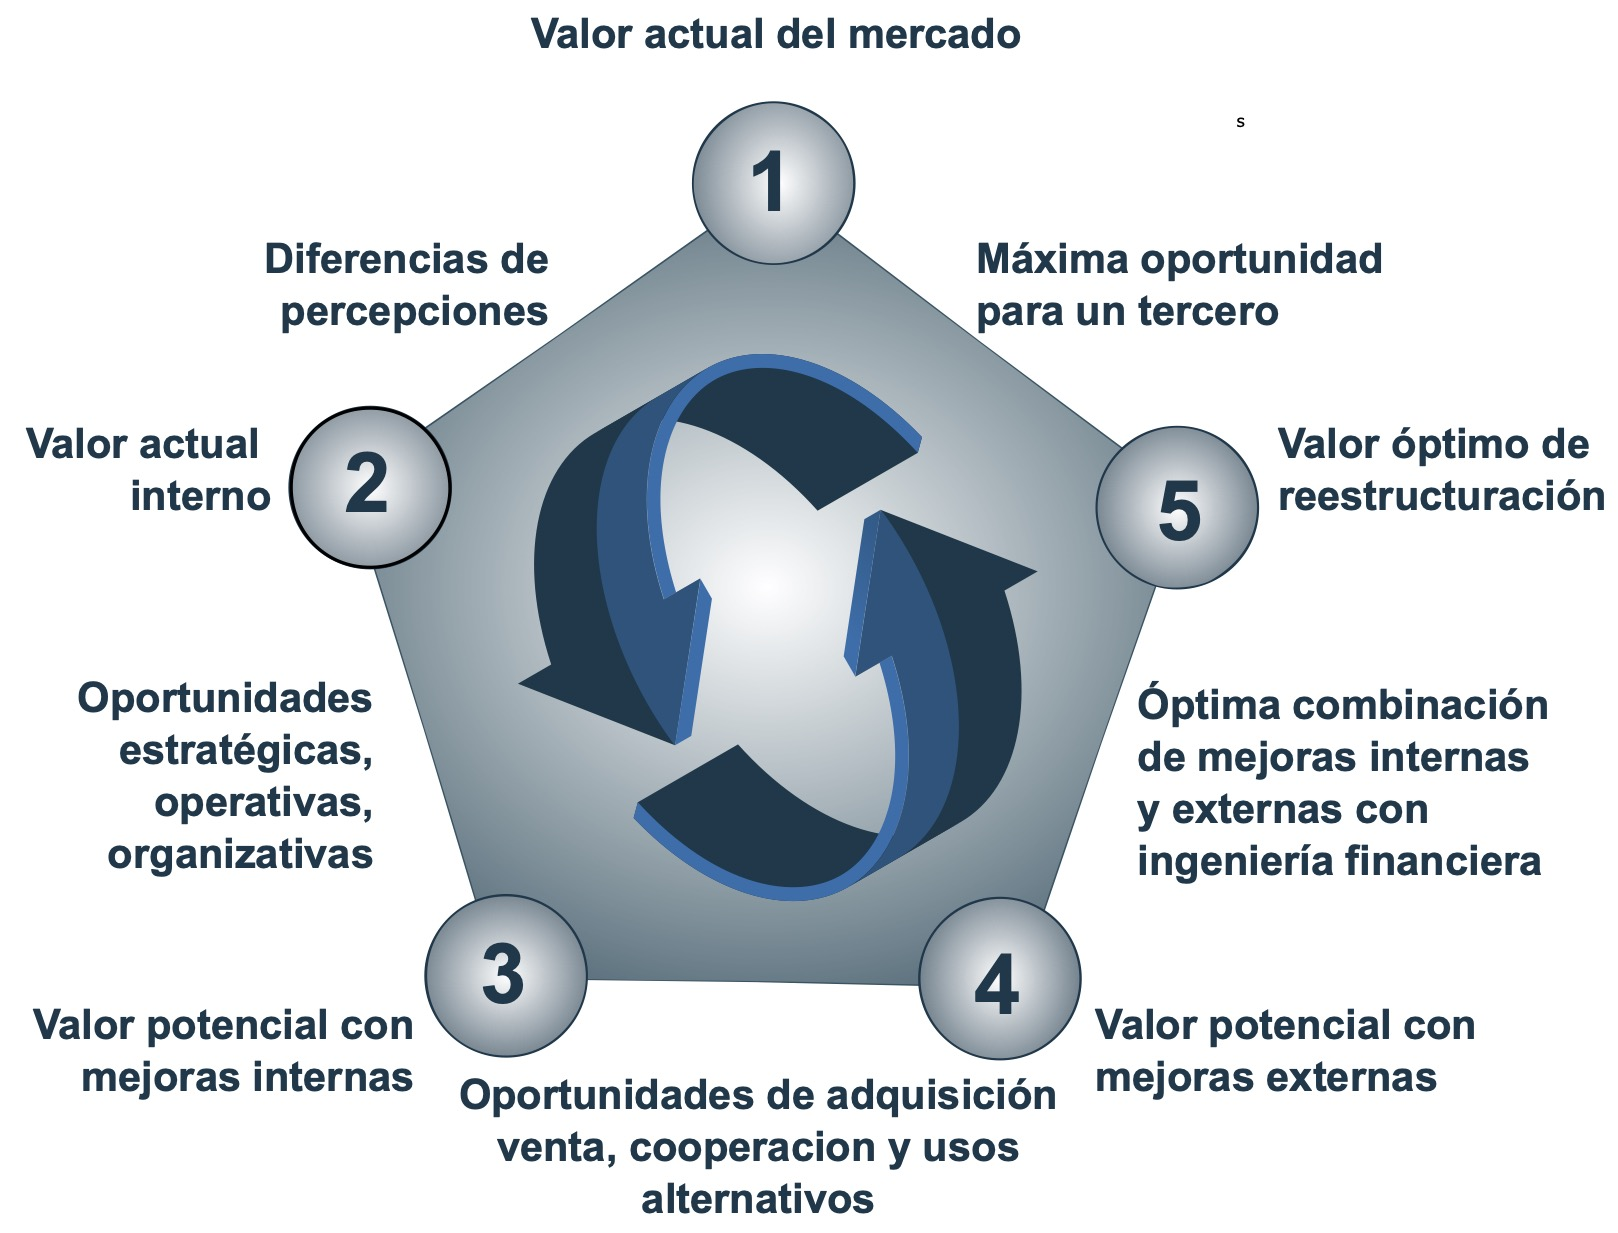
\includegraphics[width=.3\textwidth]{\rutaImagenes/pentagono.jpg}\\
\footnotesize{Fuente:Valuation. Copeland Tom, Koller Tim y Murrin Jack.\\
John Wiley \& Sons. 2000.}
\end{figure}

\end{leftcolumn}




